% This is the Reed College LaTeX thesis template. Most of the work
% for the document class was done by Sam Noble (SN), as well as this
% template. Later comments etc. by Ben Salzberg (BTS). Additional
% restructuring and APA support by Jess Youngberg (JY).
% Your comments and suggestions are more than welcome; please email
% them to cus@reed.edu
%
% See http://web.reed.edu/cis/help/latex.html for help. There are a
% great bunch of help pages there, with notes on
% getting started, bibtex, etc. Go there and read it if you're not
% already familiar with LaTeX.
%
% Any line that starts with a percent symbol is a comment.
% They won't show up in the document, and are useful for notes
% to yourself and explaining commands.
% Commenting also removes a line from the document;
% very handy for troubleshooting problems. -BTS

% As far as I know, this follows the requirements laid out in
% the 2002-2003 Senior Handbook. Ask a librarian to check the
% document before binding. -SN

%%
%% Preamble
%%
% \documentclass{<something>} must begin each LaTeX document
\documentclass[12pt,oneside]{reedthesis}
% Packages are extensions to the basic LaTeX functions. Whatever you
% want to typeset, there is probably a package out there for it.
% Chemistry (chemtex), screenplays, you name it.
% Check out CTAN to see: http://www.ctan.org/
%%
\usepackage{graphicx,latexsym}
\usepackage{amsmath}
\usepackage{amssymb,amsthm}
\usepackage{longtable,booktabs,setspace}
\usepackage{chemarr} %% Useful for one reaction arrow, useless if you're not a chem major
\usepackage[hyphens]{url}
% Added by CII
\usepackage{hyperref}
\usepackage{lmodern}
\usepackage{float}
\floatplacement{figure}{H}
% End of CII addition
\usepackage{rotating}

% Next line commented out by CII
%%% \usepackage{natbib}
% Comment out the natbib line above and uncomment the following two lines to use the new
% biblatex-chicago style, for Chicago A. Also make some changes at the end where the
% bibliography is included.
%\usepackage{biblatex-chicago}
%\bibliography{thesis}


% Added by CII (Thanks, Hadley!)
% Use ref for internal links
\renewcommand{\hyperref}[2][???]{\autoref{#1}}
\def\chapterautorefname{Chapter}
\def\sectionautorefname{Section}
\def\subsectionautorefname{Subsection}
% End of CII addition

% Added by CII
\usepackage{caption}
\captionsetup{width=5in}
% End of CII addition

% \usepackage{times} % other fonts are available like times, bookman, charter, palatino

% Syntax highlighting #22

% To pass between YAML and LaTeX the dollar signs are added by CII
\title{Exploratory Analysis of Factors Associated with Cancer Mortality\\
in the National Health and Nutrition Examination Survey Dataset}
\author{Martin Skarzynski}
% The month and year that you submit your FINAL draft TO THE LIBRARY (May or December)
\date{May 2, 2018}
\division{School of Public Health}
\advisor{Capstone Advisor: Professor Elizabeth Platz}
\institution{Johns Hopkins University}
\degree{Master of Public Health}
%If you have two advisors for some reason, you can use the following
% Uncommented out by CII
% End of CII addition

%%% Remember to use the correct department!
\department{Epidemiology}
% if you're writing a thesis in an interdisciplinary major,
% uncomment the line below and change the text as appropriate.
% check the Senior Handbook if unsure.
%\thedivisionof{The Established Interdisciplinary Committee for}
% if you want the approval page to say "Approved for the Committee",
% uncomment the next line
%\approvedforthe{Committee}

% Added by CII
%%% Copied from knitr
%% maxwidth is the original width if it's less than linewidth
%% otherwise use linewidth (to make sure the graphics do not exceed the margin)
\makeatletter
\def\maxwidth{ %
  \ifdim\Gin@nat@width>\linewidth
    \linewidth
  \else
    \Gin@nat@width
  \fi
}
\makeatother

\renewcommand{\contentsname}{Table of Contents}
% End of CII addition

\setlength{\parskip}{0pt}

% Added by CII
  %\setlength{\parskip}{\baselineskip}
  \usepackage[parfill]{parskip}

\providecommand{\tightlist}{%
  \setlength{\itemsep}{0pt}\setlength{\parskip}{0pt}}

\Acknowledgements{

}

\Dedication{

}

\Preface{

}

\Abstract{
\textbf{Context:} Large epidemiologic cohort studies, such as the
National Health and Nutrition Examination Survey (NHANES), collect
copious high-dimensional data that allow for examination of multiple
exposures in relation to a given outcome.

\textbf{Objective:} To explore the exposures measured in the Third
National Health and Nutrition Examination Survey (NHANES III) dataset in
search of factors associated with cancer mortality and to assess a
variable selection method for cancer risk prediction models.

\textbf{Methods:} We fit thousands of Cox proportional hazards models
with and without ridge penalties to randomly selected subsets of up to
50 variables. We analyzed the descriptions of NHANES III variables
provided by the National Center for Health Statistics (NCHS) and
selected 3 variables known to be related to cancer risk (age, sex and
race/ethnicity) to include in all future models. We then compared highly
significant variables (p \textless{} 10\textsuperscript{-10}) that
appeared most frequently in the Cox models and selected 5 high-frequency
highly significant variables that we used to train a new group of models
with fewer randomized variables.

\textbf{Results:} The models with fewer randomized variables
outperformed the fully randomized models in terms of concordance. Across
all of the models, the ten variables that most frequently surpassed the
p-value threshold were age, race/ethnicity, lifetime consumption of more
than 100 cigarettes, 3 variables that pertain to physical activity and 3
variables that may be related to aging.

\textbf{Conclusions:} The work described here constitutes an exploratory
analysis of the NHANES III dataset that employs an iterative strategy
for the generation of cancer risk prediction models. Looking beyond this
demonstration of a variable selection method, our ultimate goal is to
build upon previously-described cancer risk factors towards the
discovery of novel contributors to cancer risk, a deeper understanding
of cancer etiology, and an improved ability to predict cancer incidence
and mortality.
}

% End of CII addition
%%
%% End Preamble
%%
%

\usepackage{amsthm}
\newtheorem{theorem}{Theorem}[section]
\newtheorem{lemma}{Lemma}[section]
\newtheorem{corollary}{Corollary}[section]
\newtheorem{proposition}{Proposition}[section]
\newtheorem{conjecture}{Conjecture}[section]
\theoremstyle{definition}
\newtheorem{definition}{Definition}[section]
\theoremstyle{definition}
\newtheorem{example}{Example}[section]
\theoremstyle{definition}
\newtheorem{exercise}{Exercise}[section]
\theoremstyle{remark}
\newtheorem*{remark}{Remark}
\newtheorem*{solution}{Solution}
\begin{document}

% Everything below added by CII
  \maketitle

\frontmatter % this stuff will be roman-numbered
\pagestyle{empty} % this removes page numbers from the frontmatter





  \begin{abstract}
    \textbf{Context:} Large epidemiologic cohort studies, such as the
    National Health and Nutrition Examination Survey (NHANES), collect
    copious high-dimensional data that allow for examination of multiple
    exposures in relation to a given outcome.
    
    \textbf{Objective:} To explore the exposures measured in the Third
    National Health and Nutrition Examination Survey (NHANES III) dataset in
    search of factors associated with cancer mortality and to assess a
    variable selection method for cancer risk prediction models.
    
    \textbf{Methods:} We fit thousands of Cox proportional hazards models
    with and without ridge penalties to randomly selected subsets of up to
    50 variables. We analyzed the descriptions of NHANES III variables
    provided by the National Center for Health Statistics (NCHS) and
    selected 3 variables known to be related to cancer risk (age, sex and
    race/ethnicity) to include in all future models. We then compared highly
    significant variables (p \textless{} 10\textsuperscript{-10}) that
    appeared most frequently in the Cox models and selected 5 high-frequency
    highly significant variables that we used to train a new group of models
    with fewer randomized variables.
    
    \textbf{Results:} The models with fewer randomized variables
    outperformed the fully randomized models in terms of concordance. Across
    all of the models, the ten variables that most frequently surpassed the
    p-value threshold were age, race/ethnicity, lifetime consumption of more
    than 100 cigarettes, 3 variables that pertain to physical activity and 3
    variables that may be related to aging.
    
    \textbf{Conclusions:} The work described here constitutes an exploratory
    analysis of the NHANES III dataset that employs an iterative strategy
    for the generation of cancer risk prediction models. Looking beyond this
    demonstration of a variable selection method, our ultimate goal is to
    build upon previously-described cancer risk factors towards the
    discovery of novel contributors to cancer risk, a deeper understanding
    of cancer etiology, and an improved ability to predict cancer incidence
    and mortality.
  \end{abstract}

\mainmatter % here the regular arabic numbering starts
\pagestyle{fancyplain} % turns page numbering back on

\hypertarget{introduction}{%
\section*{Introduction}\label{introduction}}
\addcontentsline{toc}{section}{Introduction}

Cancer susceptibility is influenced by modifiable and non-modifiable
factors. Modifiable cancer risk factors include body mass index (BMI)
and cigarette use, whereas non-modifiable factors include age, sex,
race/ethnicity, single nucleotide polymorphisms (SNPs), and family
history of disease. According to a 2018 study by Islami and colleagues
{[}1{]}, modifiable risk factors are responsible for 42\% of all cancer
cases and 45\% of all cancer deaths. This finding suggests that cancer
prevention strategies which target modifiable risk factors have the
potential to almost halve cancer incidence and mortality in the United
States. A near two-fold reduction in cancer cases and deaths may seem
far-fetched, but cancer incidence and mortality in United Status have
been declining by \textasciitilde{}1.5\% every year from 2009-2014 and
2001-2015, respectively {[}2{]}. Taken together, these data indicate
that while tremendous progress has been made, there is still great
potential for cancer prevention approaches to decrease cancer incidence
and mortality.

The scale of cancer burden in the United States is staggering. Siegel
and colleagues estimate that in 2018 there will be 1.7 million newly
diagnosed cancer cases and roughly 600 thousand cancer deaths {[}2{]}.
Cancer risk prediction models can help policymakers and cancer
prevention practitioners develop more effective interventions and to
channel limited resources towards people at the greatest risk. To
achieve the best performance, cancer risk prediction models must include
both modifiable and non-modifiable risk factors. For example, a 2016
study by Maas and colleagues {[}3{]} demonstrated that cancer risk
prediction models based on known epidemiologic risk factors can provide
better risk stratification when genetic information such as SNPs are
included.

The challenge of cancer risk prediction is complex and will require
cancer-type specific strategies that integrate multiple types of data
and explore various modeling methods. In addition to deepening our
understanding of known cancer risk factors, it is imperative to identify
new factors that may only be meaningful in the larger context of
contributors to cancer risk. This larger context includes the collection
of genetic inheritance, called the genome, and the myriad exposures that
individuals experience during their lives, known as the exposome
{[}4{]}.

Some genetic factors and environmental exposures may be very strongly
linked to cancer. Examples of well-described genetic and environmental
cancer risk factors include TP53 gene mutation in Li-Fraumeni Syndrome
and asbestos inhalation in mesothelioma, respectively. One of the
strongest cancer risk factors is cigarette smoking. In fact, smoking was
the strongest modifiable risk factor in the 2018 study by Islami and
colleagues {[}1{]}. In this study, Islami and colleagues determined that
19\% of all cancers cases and roughly 29\% of all cancers deaths can be
attributed to cigarette smoking {[}1{]}. To look beyond known cancer
risk factors like cigarette smoking, new cancer risk prediction models
will need to detect small, but meaningful effects amid a sea of other
variables.

As part of the effort to tackle this challenge, we analyzed data from
\href{https://wwwn.cdc.gov/nchs/nhanes/nhanes3/DataFiles.aspx}{Third
National Health and Nutrition Examination Survey (NHANES III)} {[}5{]}
and the accompanying
\href{https://www.cdc.gov/nchs/data-linkage/mortality-public.htm}{National
Death Index (NDI) Public-Use Linked Mortality Files}. The first goal of
our analysis was to explore the available NHANES III data and identify
potential variables of interest for cancer mortality risk prediction.
The second goal was to define an approach for variable selection for
cancer risk prediction models.

While the current work focuses solely on NHANES III, the data
exploration and variable selection methods described here can
potentially be applied to other studies. For example, the
Atherosclerosis Risk in Communities (ARIC) study {[}6{]} and the
Framingham Heart Study (FHS) {[}7{]} are, like NHANES, large cohort
studies that do not focus on cancer, but include relevant cancer
outcomes as part of rich, multidimensional datasets. In fact, the ARIC
{[}8{]}, NHANES {[}9{]}, and FHS {[}10{]} datasets have already proven
useful for cancer research.

\hypertarget{methods}{%
\section*{Methods}\label{methods}}
\addcontentsline{toc}{section}{Methods}

The Third National Health and Nutrition Examination Survey (NHANES III)
collected data on 33,994 participants aged 2 months and older from 1988
to 1994 in the United States. The data, which include Interview, Medical
Examination, and Laboratory components, were collected and linked with
Mortality data from NDI death certificate records by the National Center
for Health Statistics (NCHS) of the Centers for Disease Control and
Prevention (CDC). From the initial pool of participants, we selected
16,404 adult (\(age \geq 18\)) participants who were cancer-free at
baseline and who had no missing values for follow-up time since
interview, NDI mortality, primary sampling units (PSU), stratification,
and sampling weight variables.

The initial publicly available dataset contained 3,544 exposures from
the Interview, Medical Examination, Laboratory, and Mortality
components. After removing variables that were non-numeric, missing any
values, only had one unique value, or had correlation to another
variable greater than 0.9, we obtained the final set of 243 exposures.
The analysis described here did not involve multiple imputation nor
utilize the NHANES III Multiply Imputed Data Set. Among the 16,404
participants, there were 964 cancer deaths and 280,891 total years of
follow-up since the initial Interview data were collected. The cancer
death and follow-up time variables were used as the outcome (survival)
in Cox proportional hazards regression analysis {[}11{]}.

NHANES III data and documentation are available on the
\href{https://wwwn.cdc.gov/nchs/nhanes/nhanes3/DataFiles.aspx}{Centers
for Disease Control (CDC) - National Center for Health Statistics (NCHS)
website}. The National Death Index (NDI) linked mortality data are
available separately on the
\href{https://www.cdc.gov/nchs/data-linkage/mortality-public.htm}{Public-Use
Linked Mortality Files webpage}. We processed the Interview, Medical
Examination, and Laboratory, and Mortality data using the
\href{https://wwwn.cdc.gov/nchs/nhanes/nhanes3/DataFiles.aspx}{SAS code
provided by NCHS}, SAS University Edition version
\texttt{9.04.01M5P09132017} on a Jupyter Notebook {[}12, 13{]} server
version \texttt{5.1.0} running with Python version \texttt{3.5.1}
{[}14{]} on the Linux {[}15{]} operating system version
\texttt{Red\ Hat\ 4.4.7-16} (with GNU Compiler Collection version
\texttt{4.4.7\ 20120313}).

We modified the SAS code to save the data as comma-separated-value
(\texttt{.csv}) files, which are available on
\href{https://figshare.com/articles/adult_csv/6210263}{FigShare}. The
SAS code files (\texttt{.sas}) and analogous Jupyter Notebook files
(\texttt{.ipynb}) are available on
\href{https://github.com/marskar/nhanes}{GitHub}. We then read the
\texttt{.csv} files into open-source R software {[}16{]} version
\texttt{3.5} using the \texttt{readr} R package {[}17{]}. R has a
vibrant community and a rich ecosystem of software packages. All of the
software packages used in this work can be accessed from the
Comprehensive R Archive Network (CRAN) {[}18{]} or from GitHub {[}19{]}
using the \texttt{devtools} package {[}20{]}.

Next, we used the \texttt{dplyr} R package {[}21{]} to 1) remove all
NHANES participant identifiers (\texttt{SEQN}) without cause of death
(\texttt{UCOD\_LEADING}) or follow-up time from interview
(\texttt{PERMTH\_INT}) variables, 2) create a cancer mortality variable
based on whether the cause of death was ``Malignant neoplasms
(\texttt{C00-C97})'', and 3) join all four datasets together by the
participant identifier variable. From the combined dataset, we removed
baseline cancer cases (using the interview variables \texttt{HAC1N} and
\texttt{HAC1O}), participants that were missing the relevant NHANES
sampling variables (\texttt{SDDPSU6}, \texttt{SDSTRA6}, and
\texttt{WTPFQX6}), variables with a time origin other than the date of
interview (e.g. \texttt{PERMTH\_EXM} ), unnecessary NHANES sampling
variables, and variables that were based on or similar to the main age
variable (such as the age in months, \texttt{HSAITMOR}). To create the
final processed dataset, we also removed highly correlated variables
(\(r \geq 0.9\)) using the \texttt{caret} R package.

NHANES III is different from many other studies, in that instead of
randomly sampling, NHANES utilizes a complex design that employs
probability-based sampling in multiple stages {[}5{]}. Methods to
analyze complex survey data using SAS, SPSS, STATA, SUDAAN, {[}22{]} and
R {[}23, 24{]} software have been described. From the final dataset, we
randomly selected 1 to 50 predictor variables and trained Cox
proportional hazards models with the \texttt{survey} R package {[}23,
24{]}, which allows for the analysis of complex survey design data using
R {[}25{]}. In half of the models, we applied ridge penalties {[}26{]}
to the predictors variables using the \texttt{survival} R Package {[}11,
27{]}. In addition to the predictor variables, the models also included
1) a ``survival object'' {[}11, 27{]} created from the event (cancer
mortality) and follow-up time variables and 2) a ``design object''
{[}24{]} created from the Primary Sampling Unit (\texttt{SDDPSU6}),
Stratification (\texttt{SDSTRA6}) and Weight (\texttt{WTPFQX6}) NHANES
sampling variables\footnote{The
  \href{https://www.cdc.gov/nchs/tutorials/NHANES/SurveyDesign/SampleDesign/intro_iii.htm}{National
  Center for Health Statistics (NCHS)} recommends the application of the
  provided sampling design variables and sampling weights in all NHANES
  analyses.}.

We then calculated statistics describing the models and the variables
they contained and saved these statistics as \texttt{.rds} files using
the \texttt{readr} package {[}17{]}. We automated the modeling and
statistical analyses using the \texttt{purrr} R package {[}28{]} and GNU
Make {[}29{]}. Specifically, the model statistics collected were
concordance {[}30{]} and Akaike Information Criterion (AIC) {[}31{]}
values, while the variable statistics were p-values, hazard ratios, and
hazard ratio confidence intervals. We unpacked the model and variable
data using the \texttt{tidyr} R package {[}32{]}.

Next, we selected 3 potential confounder variables representing age
(\texttt{HSAGEIR}) race/ethnicity (\texttt{DMAETHNR}), sex
(\texttt{HSSEX}) and repeated the modeling and statistical analysis
process described above. For the final modeling run, we chose an
additional 5 variables (\texttt{HAB1}, \texttt{HAR1}, \texttt{HAQ1},
\texttt{HAT2}, and \texttt{HAT10}) that appeared with high frequency as
highly significant (p-value \textless{} 10\textsuperscript{-10})
variables in the models we trained earlier. We joined all of the model
and variable statistics together, standardized column names using the
\texttt{stringr} {[}33{]} R package, and reordered the variable names
according to their counts using the \texttt{forcats} {[}34{]} R package.
To make the final figures, the concordance and AIC values (Figure 1),
p-values and hazard ratios (Figure 2) and the number of times each
variable appeared in the models (Figure 3) were plotted using the
\texttt{ggplot2} R package {[}35{]}.

\hypertarget{results}{%
\section*{Results}\label{results}}
\addcontentsline{toc}{section}{Results}

We present the data from thousands of Cox proportional hazards models (n
= 3789) we trained on NHANES III data in three iterative steps. The
Akaike Information Criterion (AIC) {[}31{]} and concordance values
{[}30{]} for all models are plotted in Figure 1. To better understand
the models created during the first iteration, we divided the Group 1
models into 4 subgroups (1A, 1B, 1C, and 1D) based on their AIC and
concordance values. The models from the first iteration (Figure 1;
Groups 1A-D; green, cyan, blue, purple) were fully randomized in terms
of the predictor variables that were included, while the next two
iterations (Figure 1; Groups 2-3; orange, red) consisted of models that
started with 3 and 8 non-randomized variables, respectively, before the
addition of randomly chosen variables. The 3 variables included in both
the second and third iteration were age, sex, and race/ethnicity,
whereas the final iteration contained an additional 5 variables, which
appeared frequently as highly significant (p \textless{}
10\textsuperscript{-10}) variables in the previous iterations. In all
cases, the models contained up to 50 predictor variables.

The models from the third iteration (Figure 1; Group 3; red) had the
highest concordance values overall, indicating that the addition of the
8 non-randomized predictor variables led to higher discriminatory power
between low and high-risk individuals. The gains in concordance seem to
be largely due to the addition of the age, sex, and race/ethnicity
variables as the concordance values we obtained from the second (Figure
1; Group 2; orange) and third (Figure 1; Group 3; red) iterations were
similar. Interestingly, models from the third iteration all had
concordance values of 84 or higher (Figure 1; black horizontal line),
while the range of AIC values was roughly the same in all three groups
of models (Figure 1). This finding suggests that while concordance can
differentiate between models from the three iterations, AIC by itself is
unable to make this distinction.
\begin{figure}
\centering
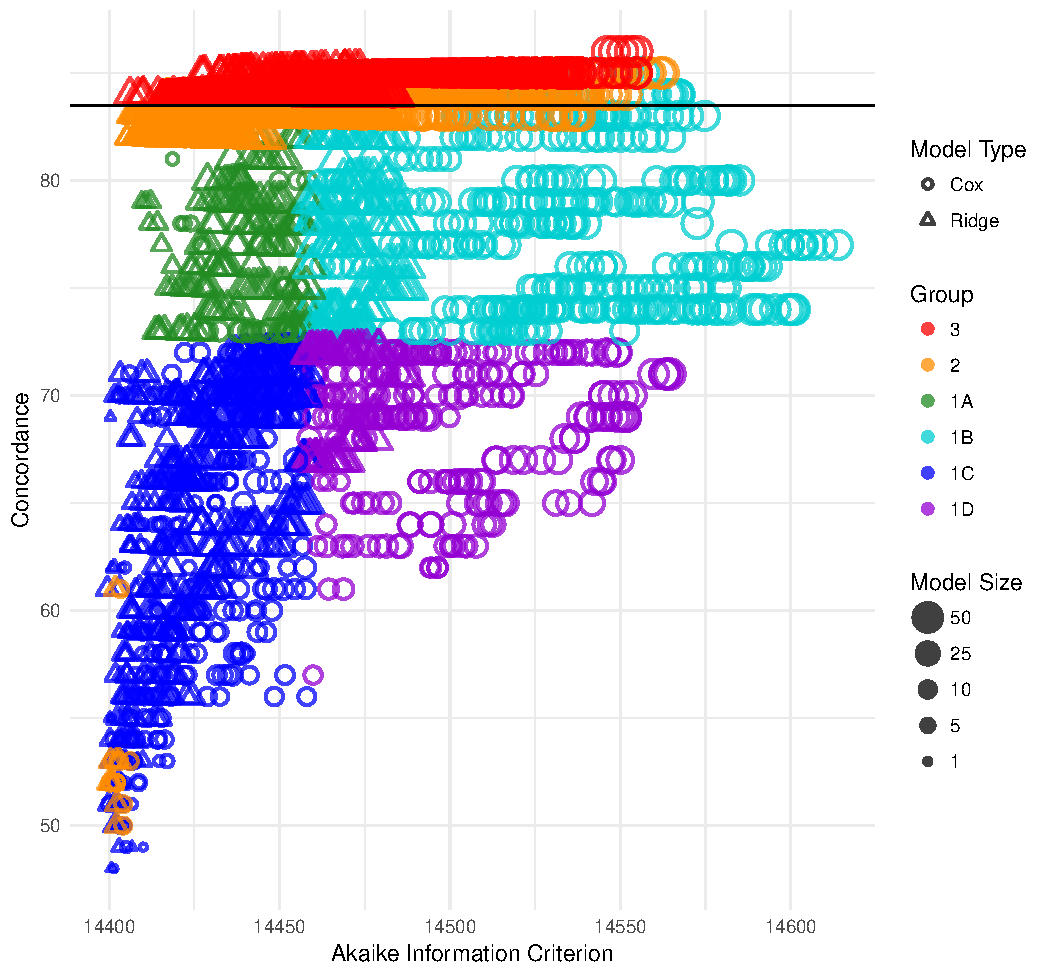
\includegraphics[width=\textwidth,height=0.6\textheight]{figure/1-quad-final.pdf}
\caption{Cancer Mortality Risk Prediction Models. \break Each point in
the scatter plot represents a Cox proportional hazards model (n = 3789).
The sizes of the points are relative to the number of variables (maximum
= 50) in each the model, while the shapes correspond to whether ridge
penalties were applied (triangle) or not (circle). The colors of points
distinguish between models that had 0 (Groups 1A-D; green, cyan, blue,
purple), 3 (Group 2; orange) or 8 (Group 3; red) non-randomized
predictor variables. Additionally, Group 1 models are further color
coded by quadrants based on concordance and Akaike Information Criterion
(AIC) values as follows: high-concordance and low-AIC (Group 1A; green),
high-concordance and high-AIC (Group 1B; cyan), low-concordance and
low-AIC (Group 1C; blue), low-concordance and high-AIC (Group 1D;
purple). All Group 3 models have concordance values of 84 or higher
(black horizontal line).}
\end{figure}
The addition of a metric like AIC is important, because it serves to
balance goodness-of-fit and model simplicity. Concordance, unlike AIC,
does not take into account the complexity of a model. As follows, larger
models tended to have higher concordance values, but also higher AIC
values. We applied ridge penalties {[}26{]}, also known as L2
regularization {[}36{]}, to half of the models from all three
iterations, and noted that ridge penalization controls this increase in
AIC as models become larger (Figure 1). The relationship between model
size and concordance appears to plateau as concordance increases (Figure
1), which suggests that the models are reaching the limit of what is
possible with the available 243 variables. Though there is almost
certainly another combination of variables that would lead to further
improvements in concordance, our approach allowed us to generate a
series of models that perform well without the need to test every
possible combination of the variables.

To choose variables to be included as non-randomized variables, we
consulted the NHANES variables descriptions available on the
\href{https://wwwn.cdc.gov/nchs/nhanes/nhanes3/DataFiles.aspx}{Centers
for Disease Control (CDC) - National Center for Health Statistics (NCHS)
website} and for the third iteration in particular we only considered
variables that had p-values lower than 10\textsuperscript{-10} (Figure
2; black horizontal line). It would be possible to introduce a threshold
for hazard ratios (Figure 2; x-axis), but this approach would tend to
select models without ridge penalties. The coefficients in ridge
penalized models are shrunk based on the penalty that is applied, which
in this case means that ridge penalized models have hazard ratios closer
to zero. While the significance and hazard ratios of variables depend on
the other variables in the model, our method allows us to survey the
landscape of p-values and hazard ratios of variables in the models
trained (Figure 2).
\begin{figure}
\centering
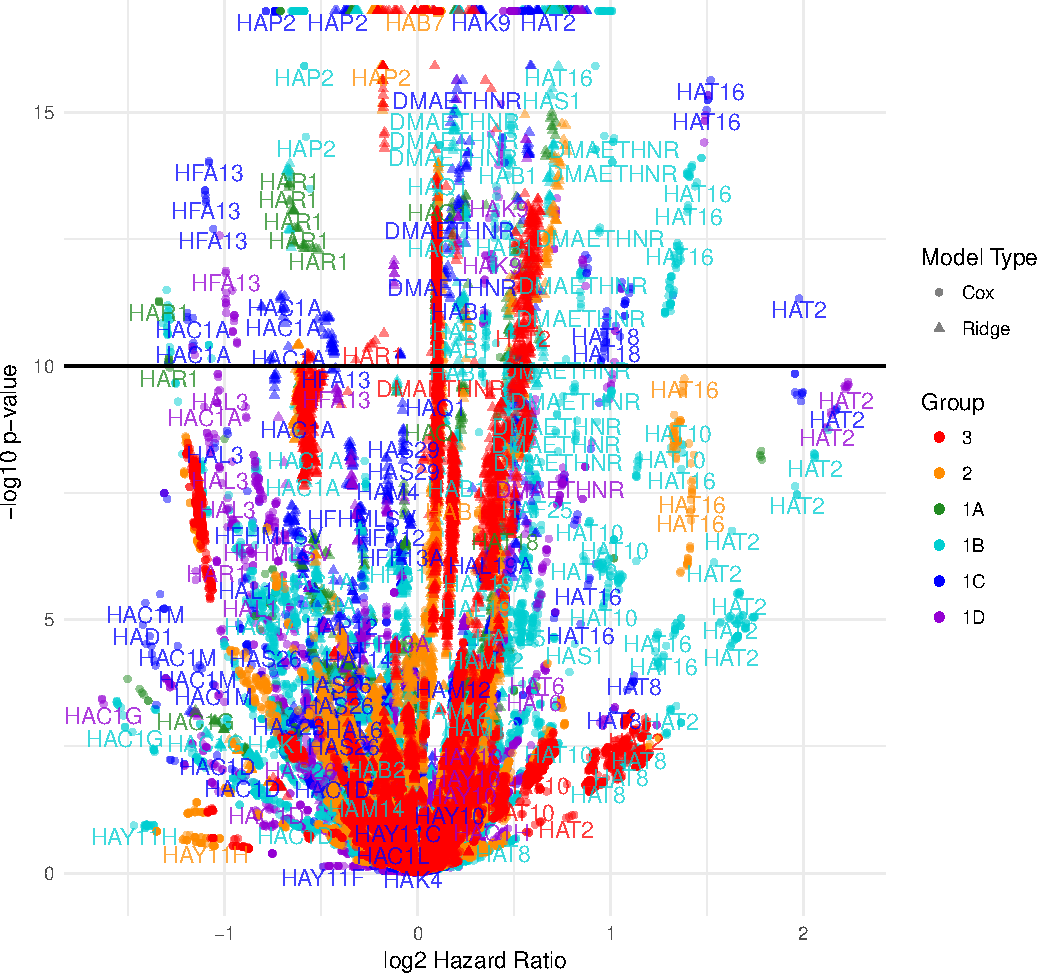
\includegraphics[width=\textwidth,height=0.6\textheight]{figure/2-volcano-final.pdf}
\caption{Lethal Cancer Risk Predictor Variables. \break Each point in
the volcano plot represents a predictor variable (n = 98787) from a Cox
proportional hazards model (n = 3789) trained on NHANES III data.
Variables are considered to be highly significant when their negative
log10 p-values (y-axis) are above 10 (black horizontal line), regardless
of their log2 hazard ratios (x-axis). The shapes of points correspond to
whether ridge penalties were applied (triangle) or not (circle). The
colors of points describe the model each variable come from as in Figure
1.}
\end{figure}
The names, median hazard ratios, counts and descriptions of the ten most
frequent highly significant variables are summarized in Table 1. The
variable descriptions are based on the
\href{https://wwwn.cdc.gov/nchs/nhanes/nhanes3/DataFiles.aspx}{documentation
on the NHANES III website}. Each row in Table 1 represents one of the
ten predictor variables that appeared most frequently as highly
significant (p \textless{} 10\textsuperscript{-10}) variables in the Cox
models (n = 3789) trained on NHANES III data. The median hazard ratio
(HR) and count (n) statistics describe only highly significant
variables. The variable that appeared most frequently as highly
significant across all of the models was age (Figure 3;
\texttt{HSAGEIR}). When focusing on the Group 1 models (Figure 3; Groups
1A-D; green, cyan, blue, purple), the most frequent highly significant
variable was an interview question regarding dental health (Figure 3;
\texttt{HAQ1}). The other top 10 high-frequency highly significant
variables were race/ethnicity (\texttt{DMAETHNR}), lifetime consumption
of more than 100 cigarettes (\texttt{HAR1}), 3 variables related to
physical activity (\texttt{HAT2}, \texttt{HAT10}, \texttt{HAT16}), and 3
variables that may be associated to aging (\texttt{HAB7}, \texttt{HAK9},
and \texttt{HAP2}). Interestingly, one of the variables, ``In the past
12 months, how many times were you in a nursing home?'' (\texttt{HAB7}),
was present as a highly significant variable only in the second and
third groups.
\begin{figure}
\centering
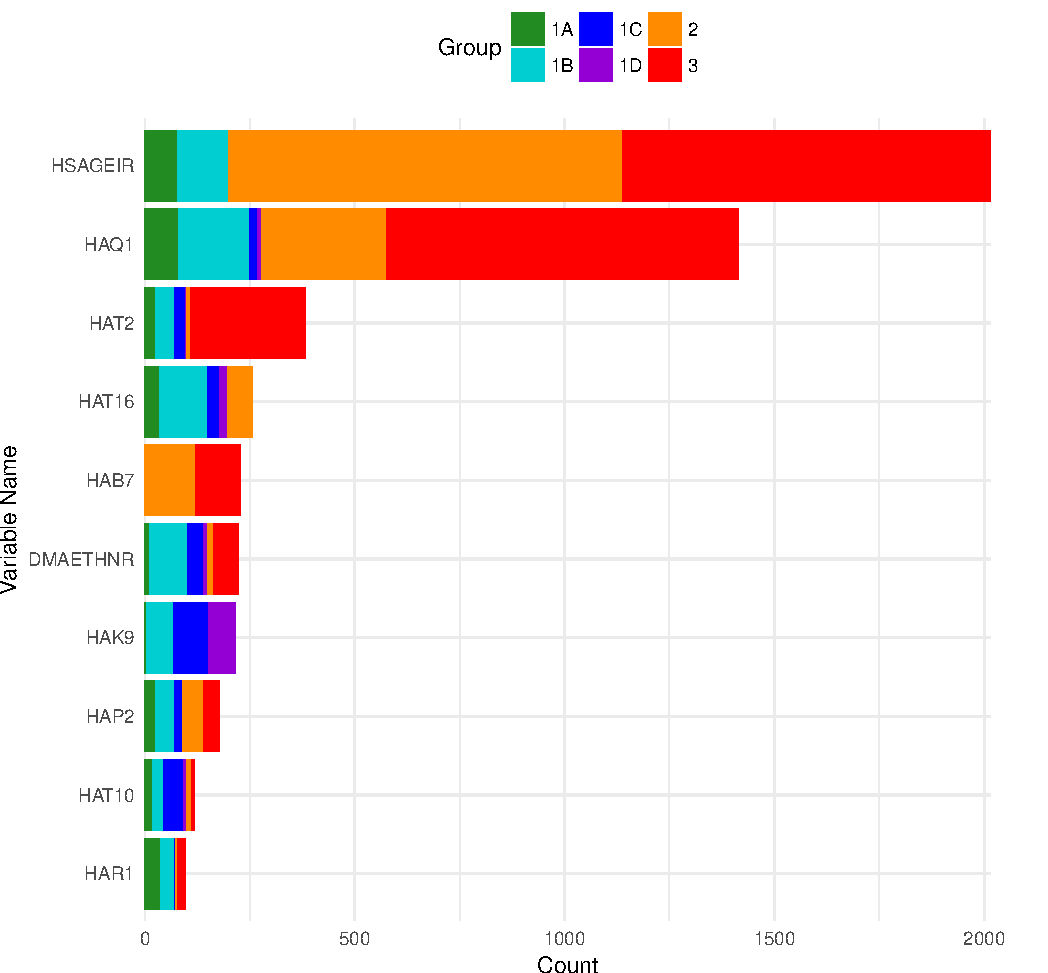
\includegraphics[width=\textwidth,height=0.6\textheight]{figure/3-varbar-final.pdf}
\caption{Highly Significant Predictor Variable Frequency. \break Each
bar represents the number of times (x-axis) a variables (y-axis)
appeared in the 3789 Cox proportional hazards models. The colors of bars
correspond to the proportion of variables that orginiated from each of
the four Group 1 subgroups (Groups 1A-D; green, cyan, blue, purple) and
the subsequent iterations (Groups 2-3; orange, red), as in Figures 1 and
2.}
\end{figure}
\begin{longtable}[]{@{}llll@{}}
\caption{The Ten Most Frequent Highly Significant
Variables}\tabularnewline
\toprule
\begin{minipage}[b]{0.21\columnwidth}\raggedright
Name\strut
\end{minipage} & \begin{minipage}[b]{0.23\columnwidth}\raggedright
Median HR\strut
\end{minipage} & \begin{minipage}[b]{0.12\columnwidth}\raggedright
n\strut
\end{minipage} & \begin{minipage}[b]{0.33\columnwidth}\raggedright
Description\strut
\end{minipage}\tabularnewline
\midrule
\endfirsthead
\toprule
\begin{minipage}[b]{0.21\columnwidth}\raggedright
Name\strut
\end{minipage} & \begin{minipage}[b]{0.23\columnwidth}\raggedright
Median HR\strut
\end{minipage} & \begin{minipage}[b]{0.12\columnwidth}\raggedright
n\strut
\end{minipage} & \begin{minipage}[b]{0.33\columnwidth}\raggedright
Description\strut
\end{minipage}\tabularnewline
\midrule
\endhead
\begin{minipage}[t]{0.21\columnwidth}\raggedright
HSAGEIR\strut
\end{minipage} & \begin{minipage}[t]{0.23\columnwidth}\raggedright
1.04\strut
\end{minipage} & \begin{minipage}[t]{0.12\columnwidth}\raggedright
2016\strut
\end{minipage} & \begin{minipage}[t]{0.33\columnwidth}\raggedright
Age in Years\strut
\end{minipage}\tabularnewline
\begin{minipage}[t]{0.21\columnwidth}\raggedright
HAQ1\strut
\end{minipage} & \begin{minipage}[t]{0.23\columnwidth}\raggedright
1.07\strut
\end{minipage} & \begin{minipage}[t]{0.12\columnwidth}\raggedright
1415\strut
\end{minipage} & \begin{minipage}[t]{0.33\columnwidth}\raggedright
How would you describe the condition of your natural teeth (excellent,
very good, good, fair or poor)?\strut
\end{minipage}\tabularnewline
\begin{minipage}[t]{0.21\columnwidth}\raggedright
HAT2\strut
\end{minipage} & \begin{minipage}[t]{0.23\columnwidth}\raggedright
1.50\strut
\end{minipage} & \begin{minipage}[t]{0.12\columnwidth}\raggedright
384\strut
\end{minipage} & \begin{minipage}[t]{0.33\columnwidth}\raggedright
In the past month, did you jog or run?\strut
\end{minipage}\tabularnewline
\begin{minipage}[t]{0.21\columnwidth}\raggedright
HAT16\strut
\end{minipage} & \begin{minipage}[t]{0.23\columnwidth}\raggedright
1.67\strut
\end{minipage} & \begin{minipage}[t]{0.12\columnwidth}\raggedright
256\strut
\end{minipage} & \begin{minipage}[t]{0.33\columnwidth}\raggedright
In the past month, did you lift weights?\strut
\end{minipage}\tabularnewline
\begin{minipage}[t]{0.21\columnwidth}\raggedright
HAB7\strut
\end{minipage} & \begin{minipage}[t]{0.23\columnwidth}\raggedright
0.99\strut
\end{minipage} & \begin{minipage}[t]{0.12\columnwidth}\raggedright
228\strut
\end{minipage} & \begin{minipage}[t]{0.33\columnwidth}\raggedright
In the past 12 months, how many times were you in a nursing home?\strut
\end{minipage}\tabularnewline
\begin{minipage}[t]{0.21\columnwidth}\raggedright
DMAETHNR\strut
\end{minipage} & \begin{minipage}[t]{0.23\columnwidth}\raggedright
1.14\strut
\end{minipage} & \begin{minipage}[t]{0.12\columnwidth}\raggedright
224\strut
\end{minipage} & \begin{minipage}[t]{0.33\columnwidth}\raggedright
Race/Ethnicity\strut
\end{minipage}\tabularnewline
\begin{minipage}[t]{0.21\columnwidth}\raggedright
HAK9\strut
\end{minipage} & \begin{minipage}[t]{0.23\columnwidth}\raggedright
1.23\strut
\end{minipage} & \begin{minipage}[t]{0.12\columnwidth}\raggedright
216\strut
\end{minipage} & \begin{minipage}[t]{0.33\columnwidth}\raggedright
How many times per night do you usually get up to urinate?\strut
\end{minipage}\tabularnewline
\begin{minipage}[t]{0.21\columnwidth}\raggedright
HAP2\strut
\end{minipage} & \begin{minipage}[t]{0.23\columnwidth}\raggedright
0.81\strut
\end{minipage} & \begin{minipage}[t]{0.12\columnwidth}\raggedright
179\strut
\end{minipage} & \begin{minipage}[t]{0.33\columnwidth}\raggedright
Do you use glasses, contacts, or both?\strut
\end{minipage}\tabularnewline
\begin{minipage}[t]{0.21\columnwidth}\raggedright
HAT10\strut
\end{minipage} & \begin{minipage}[t]{0.23\columnwidth}\raggedright
1.43\strut
\end{minipage} & \begin{minipage}[t]{0.12\columnwidth}\raggedright
119\strut
\end{minipage} & \begin{minipage}[t]{0.33\columnwidth}\raggedright
In the past month, did you do other dancing?\strut
\end{minipage}\tabularnewline
\begin{minipage}[t]{0.21\columnwidth}\raggedright
HAR1\strut
\end{minipage} & \begin{minipage}[t]{0.23\columnwidth}\raggedright
0.63\strut
\end{minipage} & \begin{minipage}[t]{0.12\columnwidth}\raggedright
96\strut
\end{minipage} & \begin{minipage}[t]{0.33\columnwidth}\raggedright
Have you smoked at least 100 cigarettes during your entire life?\strut
\end{minipage}\tabularnewline
\bottomrule
\end{longtable}
The ranks of variables shown in Table 1 are determined by counts from
all 3789 models, and thus are heavily influenced by the fact that some
variables are included in all Group 2 (\texttt{HSAGEIR},
\texttt{DMAETHNR}, and \texttt{HSSEX}) and Group 3 (\texttt{HSAGEIR},
\texttt{DMAETHNR}, \texttt{HSSEX}, \texttt{HAB1}, \texttt{HAR1},
\texttt{HAQ1}, \texttt{HAT2}, and \texttt{HAT10}) models. Table 1
therefore serves as a summary of all three iterations of modeling and
statistical analysis. Rather than selecting the variables with the
lowest p-values or highest hazard ratios, we chose to follow a strategy
that counts the number of times a variable's significance crosses a
p-value threshold. This type of frequency-based ranking of variables can
be used to both guide future variable selection decisions and assess
previous steps in the model building process.

\hypertarget{discussion}{%
\section*{Discussion}\label{discussion}}
\addcontentsline{toc}{section}{Discussion}

To obtain a better understanding of how variables for cancer risk
prediction models can be selected, we utilized an iterative strategy to
explore the variables in the NHANES III dataset. As part of this
strategy, we randomly generated a large number of Cox proportional
hazards models to guide the training of new models with fewer randomly
chosen variables in future iterations. This method is akin to forward
subset selection {[}37{]} in that models are built up variable by
variable, but differs in that models are not assessed with the addition
of each new variable. In fact, the method we employed does not take
model performance metrics into consideration when selecting variables.
To inform variable selection in subsequent iterations, we instead
focused on the frequency with which variables had p-values below
10\textsuperscript{-10}.

In essence, our current approach aggregates information from across many
models into a single statistic per variable. Variable selection
decisions could be informed by another statistic or a combination of
other statistics. For example, the significance threshold (p \textless{}
10\textsuperscript{-10}) we put in place was arbitrary and our method
could be used with a different threshold value, a different metric or a
combination of different thresholds. For example, variables could be
selected based on the number of times the absolute value of their hazard
ratio crosses a certain threshold. Model statistics could also be
employed for thresholds as the concordance, Akaike Information Criterion
(AIC) and other model performance metrics remain associated with
variables throughout all steps in the process.

In addition to changing the variable selection threshold, the method
described here could be adapted to use regularization techniques other
than ridge regression {[}26{]} and models other than Cox proportional
hazards models. In terms of regularization, survival analyses can be
done with lasso {[}38{]} penalties or a combination of ridge and lasso
penalties, which is known as Elastic Net {[}39{]}. As for possible
modeling algorithms to explore in the future include tree-based models
such as survival tree {[}40{]}, survival random forest models {[}41{]}.
Tree-based models are easy to interpret and allow for the quantification
of the proportion of variance explained by variables included in the
model. Another statistical method called boosting, for example
\texttt{XGBoost} {[}42{]}, can be used to compute F-scores representing
the importance of each variable.

Regardless of the algorithms or thresholds used, the final result of our
approach is a new dataset of statistics that describe models and
variables across all iterations. This new dataset could be merged with
text data, such as the
\href{https://wwwn.cdc.gov/nchs/nhanes/nhanes3/DataFiles.aspx}{NHANES
III variable descriptions provided by the National Center for Health
Statistics}, and employ Natural Language Processing (NLP) {[}43{]}
techniques to add further the information related to the models and
variables in the dataset. For example, NLP techniques could be used to
classify variables into categories, such as physical activity or
nutrition, based on their descriptions. All of this information could
then be combined with domain knowledge to steer the variable selection
process.

The types of variables that were ranked highest in our present analysis
(age, race/ethnicity, smoking and physical activity) are all already
known to be strongly associated with cancer death. While obtaining an
unsurprising result serves to confirm the validity of our method, the
main objective of this work is to provide insight that will lead to the
identification of new cancer risk factors. To this end, our method will
have to be refined to detect variables that weakly contribute to cancer
risk or whose contribution is context-specific.

We demonstrated the ability of our method to generate models that
predict lethal cancer risk in the NHANES III dataset with high accuracy
(\(concordance \geq 84\)). It remains to be seen, whether our approach
could be generalizable to other studies and other outcomes. NHANES III
does not include cancer-type-specific mortality data, but other studies,
such as the Atherosclerosis Risk in Communities study (ARIC) {[}6, 8{]},
may provide the opportunity to generate and assess models that predict
mortality or incidence of a specific type of cancer. As a continuation
of this project, we will expand the methods described here into a
general methodology that can be applied beyond NHANES III to other
large, high-dimensional cohort studies. In addition to generalization to
other studies, future work on this project will include the creation of
a software package that encapsulates all of the relevant code and a
graphical user interface that facilitates data exploration, model
parameter modification and variable selection.

\hypertarget{connections-to-mph-goals-analysis}{%
\section*{Connections to MPH Goals
Analysis}\label{connections-to-mph-goals-analysis}}
\addcontentsline{toc}{section}{Connections to MPH Goals Analysis}

My Master of Public Health (MPH) experience at Johns Hopkins has been
absolutely transformative. Though I started my MPH studies with a strong
background in science, I had no experience with public health or
population science. Similarly, while I was comfortable with R
programming, I did not know the first thing about survey data, let alone
how to conduct complex survey analyses in R. In my Goals Analysis Plan,
I outlined my goal of broadening my horizons in three areas: 1)
substantive expertise (domain knowledge), 2) statistics and mathematics,
and 3) technical (programming) skills {[}44{]}. Looking back on the
progress I made during my MPH studies, I am confident that I have
achieved my goals. This Research Report Capstone Project is testament to
the skills I honed and the knowledge I gained over the past year. I look
forward to building upon this Capstone as I continue my career in cancer
prevention research.

\hypertarget{references}{%
\section*{References}\label{references}}
\addcontentsline{toc}{section}{References}

\hypertarget{refs}{}
\leavevmode\hypertarget{ref-Islami_2018}{}%
1. Islami F, Sauer AG, Miller KD, Siegel RL, Fedewa SA, Jacobs EJ, et
al. Proportion and number of cancer cases and deaths attributable to
potentially modifiable risk factors in the united states. CA: A Cancer
Journal for Clinicians. 2018;68:31--54.
doi:\href{https://doi.org/10.3322/caac.21440}{10.3322/caac.21440}.

\leavevmode\hypertarget{ref-Siegel_2018}{}%
2. Siegel RL, Miller KD, Jemal A. Cancer statistics, 2018. CA: A Cancer
Journal for Clinicians. 2018;68:7--30.
doi:\href{https://doi.org/10.3322/caac.21442}{10.3322/caac.21442}.

\leavevmode\hypertarget{ref-Maas_2016}{}%
3. Maas P, Barrdahl M, Joshi AD, Auer PL, Gaudet MM, Milne RL, et al.
Breast cancer risk from modifiable and nonmodifiable risk factors among
white women in the united states. JAMA Oncology. 2016;2:1295.
doi:\href{https://doi.org/10.1001/jamaoncol.2016.1025}{10.1001/jamaoncol.2016.1025}.

\leavevmode\hypertarget{ref-Wild_2005}{}%
4. Wild CP. Complementing the genome with an "exposome": The outstanding
challenge of environmental exposure measurement in molecular
epidemiology. Cancer Epidemiology Biomarkers \& Prevention.
2005;14:1847--50.
doi:\href{https://doi.org/10.1158/1055-9965.epi-05-0456}{10.1158/1055-9965.epi-05-0456}.

\leavevmode\hypertarget{ref-nhanes_1994}{}%
5. National Center for Health Statistics (NCHS), others. Plan and
operation of the third national health and nutrition examination survey,
1988-94. Series 1: Programs and collection procedures. Vital Health
Statistics, Series 1. 1994;32:1--407.

\leavevmode\hypertarget{ref-ARIC_1989}{}%
6. The Atherosclerosis Risk In Communities (ARIC) study: Design and
objectives. American Journal of Epidemiology. 1989;129:687--702.
doi:\href{https://doi.org/10.1093/oxfordjournals.aje.a115184}{10.1093/oxfordjournals.aje.a115184}.

\leavevmode\hypertarget{ref-Mahmood_2014}{}%
7. Mahmood SS, Levy D, Vasan RS, Wang TJ. The Framingham Heart Study and
the epidemiology of cardiovascular disease: A historical perspective.
The Lancet. 2014;383:999--1008.
doi:\href{https://doi.org/10.1016/S0140-6736(13)61752-3}{10.1016/S0140-6736(13)61752-3}.

\leavevmode\hypertarget{ref-Joshu_2017}{}%
8. Joshu CE, Barber JR, Coresh J, Couper DJ, Mosley TH, Vitolins MZ, et
al. Enhancing the infrastructure of the Atherosclerosis Risk in
Communities (ARIC) study for cancer epidemiology research: ARIC cancer.
Cancer Epidemiology Biomarkers \& Prevention. 2017;27:295--305.
doi:\href{https://doi.org/10.1158/1055-9965.epi-17-0696}{10.1158/1055-9965.epi-17-0696}.

\leavevmode\hypertarget{ref-Freedman_2010}{}%
9. Freedman DM, Looker AC, Abnet CC, Linet MS, Graubard BI. Serum
25-Hydroxyvitamin D and Cancer Mortality in the NHANES III Study
(1988--2006). Cancer Research. 2010;70:8587--97.
doi:\href{https://doi.org/10.1158/0008-5472.CAN-10-1420}{10.1158/0008-5472.CAN-10-1420}.

\leavevmode\hypertarget{ref-Kreger_1991}{}%
10. Kreger BE, Splansky GL, Schatzkin A. The cancer experience in the
framingham heart study cohort. Cancer. 1991;67:1--6.
doi:\href{https://doi.org/10.1002/1097-0142(19910101)67:1\%3C1::AID-CNCR2820670102\%3E3.0.CO;2-W}{10.1002/1097-0142(19910101)67:1\textless{}1::AID-CNCR2820670102\textgreater{}3.0.CO;2-W}.

\leavevmode\hypertarget{ref-Therneau_2000}{}%
11. Terry M. Therneau, Patricia M. Grambsch. Modeling survival data:
Extending the Cox model. New York: Springer; 2000.

\leavevmode\hypertarget{ref-Kluyver_2016}{}%
12. Kluyver T, Ragan-Kelley B, Pérez F, Granger BE, Bussonnier M,
Frederic J, et al. Jupyter notebooks - A publishing format for
reproducible computational workflows. In: ELPUB. 2016. pp. 87--90.

\leavevmode\hypertarget{ref-Perez_2007}{}%
13. Pérez F, Granger BE. IPython: A System for Interactive Scientific
Computing. Computing in Science \& Engineering. 2007;9:21--9.

\leavevmode\hypertarget{ref-python_2003}{}%
14. Van Rossum G, Drake FL. Python language reference manual. Network
Theory; 2003.

\leavevmode\hypertarget{ref-Torvalds_2001}{}%
15. Torvalds L, Diamond D. Just for fun: The story of an accidental
revolutionary. Harper Business; 2001.

\leavevmode\hypertarget{ref-Rcore_2018}{}%
16. R Core Team. R: A language and environment for statistical
computing. Vienna, Austria: R Foundation for Statistical Computing;
2018. \url{https://www.R-project.org/}.

\leavevmode\hypertarget{ref-readr_2017}{}%
17. Wickham H, Hester J, Francois R. Readr: Read rectangular text data.
2017. \url{https://CRAN.R-project.org/package=readr}.

\leavevmode\hypertarget{ref-Hornik_2017}{}%
18. Hornik K. R FAQ. 2017.
\url{https://CRAN.R-project.org/doc/FAQ/R-FAQ.html}.

\leavevmode\hypertarget{ref-Vuorre_2018}{}%
19. Vuorre M, Curley JP. Curating research assets: A tutorial on the git
version control system. Advances in Methods and Practices in
Psychological Science. 2018;0:2515245918754826.
doi:\href{https://doi.org/10.1177/2515245918754826}{10.1177/2515245918754826}.

\leavevmode\hypertarget{ref-devtools_2018}{}%
20. Wickham H, Hester J, Chang W. Devtools: Tools to make developing R
packages easier. 2018.
\url{https://CRAN.R-project.org/package=devtools}.

\leavevmode\hypertarget{ref-dplyr_2017}{}%
21. Wickham H, Francois R, Henry L, Müller K. Dplyr: A grammar of data
manipulation. 2017. \url{https://CRAN.R-project.org/package=dplyr}.

\leavevmode\hypertarget{ref-Siller_2006}{}%
22. Siller AB, Tompkins L. The big four: Analyzing complex sample survey
data using SAS, SPSS, STATA, and SUDAAN. In: Proceedings of the
thirty-first annual sas users group international conference. SAS
Institute Inc; 2006. pp. 26--9.

\leavevmode\hypertarget{ref-Lumley_2004}{}%
23. Lumley T. Analysis of complex survey samples. Journal of Statistical
Software. 2004;9:1--19.

\leavevmode\hypertarget{ref-survey_2017}{}%
24. Lumley T. Survey: Analysis of complex survey samples. 2017.
\url{https://CRAN.R-project.org/package=survey}.

\leavevmode\hypertarget{ref-Lumley_2011}{}%
25. Lumley T. Complex surveys: A guide to analysis using R. John Wiley
\& Sons; 2011.

\leavevmode\hypertarget{ref-Hoerl_1970}{}%
26. Hoerl AE, Kennard RW. Ridge regression: Biased estimation for
nonorthogonal problems. Technometrics. 1970;12:55.
doi:\href{https://doi.org/10.2307/1267351}{10.2307/1267351}.

\leavevmode\hypertarget{ref-survival_2015}{}%
27. Therneau TM. A package for survival analysis in s. 2015.
\url{https://CRAN.R-project.org/package=survival}.

\leavevmode\hypertarget{ref-purrr_2017}{}%
28. Henry L, Wickham H. Purrr: Functional programming tools. 2017.
\url{https://CRAN.R-project.org/package=purrr}.

\leavevmode\hypertarget{ref-Mecklenburg_2004}{}%
29. Mecklenburg R. Managing projects with GNU make: The power of GNU
make for building anything. "O'Reilly Media, Inc."; 2004.

\leavevmode\hypertarget{ref-Bozdogan_1987}{}%
30. Bozdogan H. Model selection and Akaike's information criterion
(AIC): the general theory and its analytical extensions. Psychometrika.
1987;52:345--70.

\leavevmode\hypertarget{ref-Gonen_2005}{}%
31. Gönen M, Heller G. Concordance probability and discriminatory power
in proportional hazards regression. Biometrika. 2005;92:965--70.

\leavevmode\hypertarget{ref-tidyr_2018}{}%
32. Wickham H, Henry L. Tidyr: Easily tidy data with 'spread()' and
'gather()' f unctions. 2018.
\url{https://CRAN.R-project.org/package=tidyr}.

\leavevmode\hypertarget{ref-stringr_2018}{}%
33. Wickham H. Stringr: Simple, consistent wrappers for common string o
perations. 2018. \url{https://CRAN.R-project.org/package=stringr}.

\leavevmode\hypertarget{ref-forcats_2018}{}%
34. Wickham H. Forcats: Tools for working with categorical variables (f
actors). 2018. \url{https://CRAN.R-project.org/package=forcats}.

\leavevmode\hypertarget{ref-gglot2_2009}{}%
35. Wickham H. Ggplot2: Elegant graphics for data analysis.
Springer-Verlag New York; 2009. \url{http://ggplot2.org}.

\leavevmode\hypertarget{ref-Ng_2004}{}%
36. Ng AY. Feature selection, l1 vs. L2 regularization, and rotational
invariance. In: Proceedings of the twenty-first international conference
on machine learning. ACM; 2004. p. 78.

\leavevmode\hypertarget{ref-Kohavi_1997}{}%
37. Kohavi R, John GH. Wrappers for feature subset selection. Artificial
intelligence. 1997;97:273--324.

\leavevmode\hypertarget{ref-Tibshirani_1997}{}%
38. Tibshirani R. The lasso method for variable selection in the Cox
model. Statistics in medicine. 1997;16:385--95.

\leavevmode\hypertarget{ref-Zou_2005}{}%
39. Zou H, Hastie T. Regularization and variable selection via the
elastic net. Journal of the Royal Statistical Society: Series B
(Statistical Methodology). 2005;67:301--20.

\leavevmode\hypertarget{ref-rpart_2017}{}%
40. Therneau T, Atkinson B, Ripley B. Rpart: Recursive partitioning and
regression trees. 2017. \url{https://CRAN.R-project.org/package=rpart}.

\leavevmode\hypertarget{ref-Ishwaran_2008}{}%
41. Ishwaran H, Kogalur UB, Blackstone EH, Lauer MS. Random survival
forests. The Annals of Applied Statistics. 2008;2:841--60.
doi:\href{https://doi.org/10.1214/08-aoas169}{10.1214/08-aoas169}.

\leavevmode\hypertarget{ref-Chen_2016}{}%
42. Chen T, Guestrin C. XGBoost. In: Proceedings of the 22nd ACM SIGKDD
international conference on knowledge discovery and data mining - KDD
16. ACM Press; 2016.
doi:\href{https://doi.org/10.1145/2939672.2939785}{10.1145/2939672.2939785}.

\leavevmode\hypertarget{ref-Chowdhury_2003}{}%
43. Chowdhury GG. Natural language processing. Annual review of
information science and technology. 2003;37:51--89.

\leavevmode\hypertarget{ref-Conway_2010}{}%
44. Conway D. The data science venn diagram. 2010.
\url{http://drewconway.com/zia/2013/3/26/the-data-science-venn-diagram}.


% Index?

\end{document}
